\documentclass[handout]{ximera}
%handout:  for handout version with no solutions or instructor notes
%handout,instructornotes:  for instructor version with just problems and notes, no solutions
%noinstructornotes:  shows only problem and solutions

%% handout
%% space
%% newpage
%% numbers
%% nooutcomes

%I added the commands here so that I would't have to keep looking them up
%\newcommand{\RR}{\mathbb R}
%\renewcommand{\d}{\,d}
%\newcommand{\dd}[2][]{\frac{d #1}{d #2}}
%\renewcommand{\l}{\ell}
%\newcommand{\ddx}{\frac{d}{dx}}
%\everymath{\displaystyle}
%\newcommand{\dfn}{\textbf}
%\newcommand{\eval}[1]{\bigg[ #1 \bigg]}

%\begin{image}
%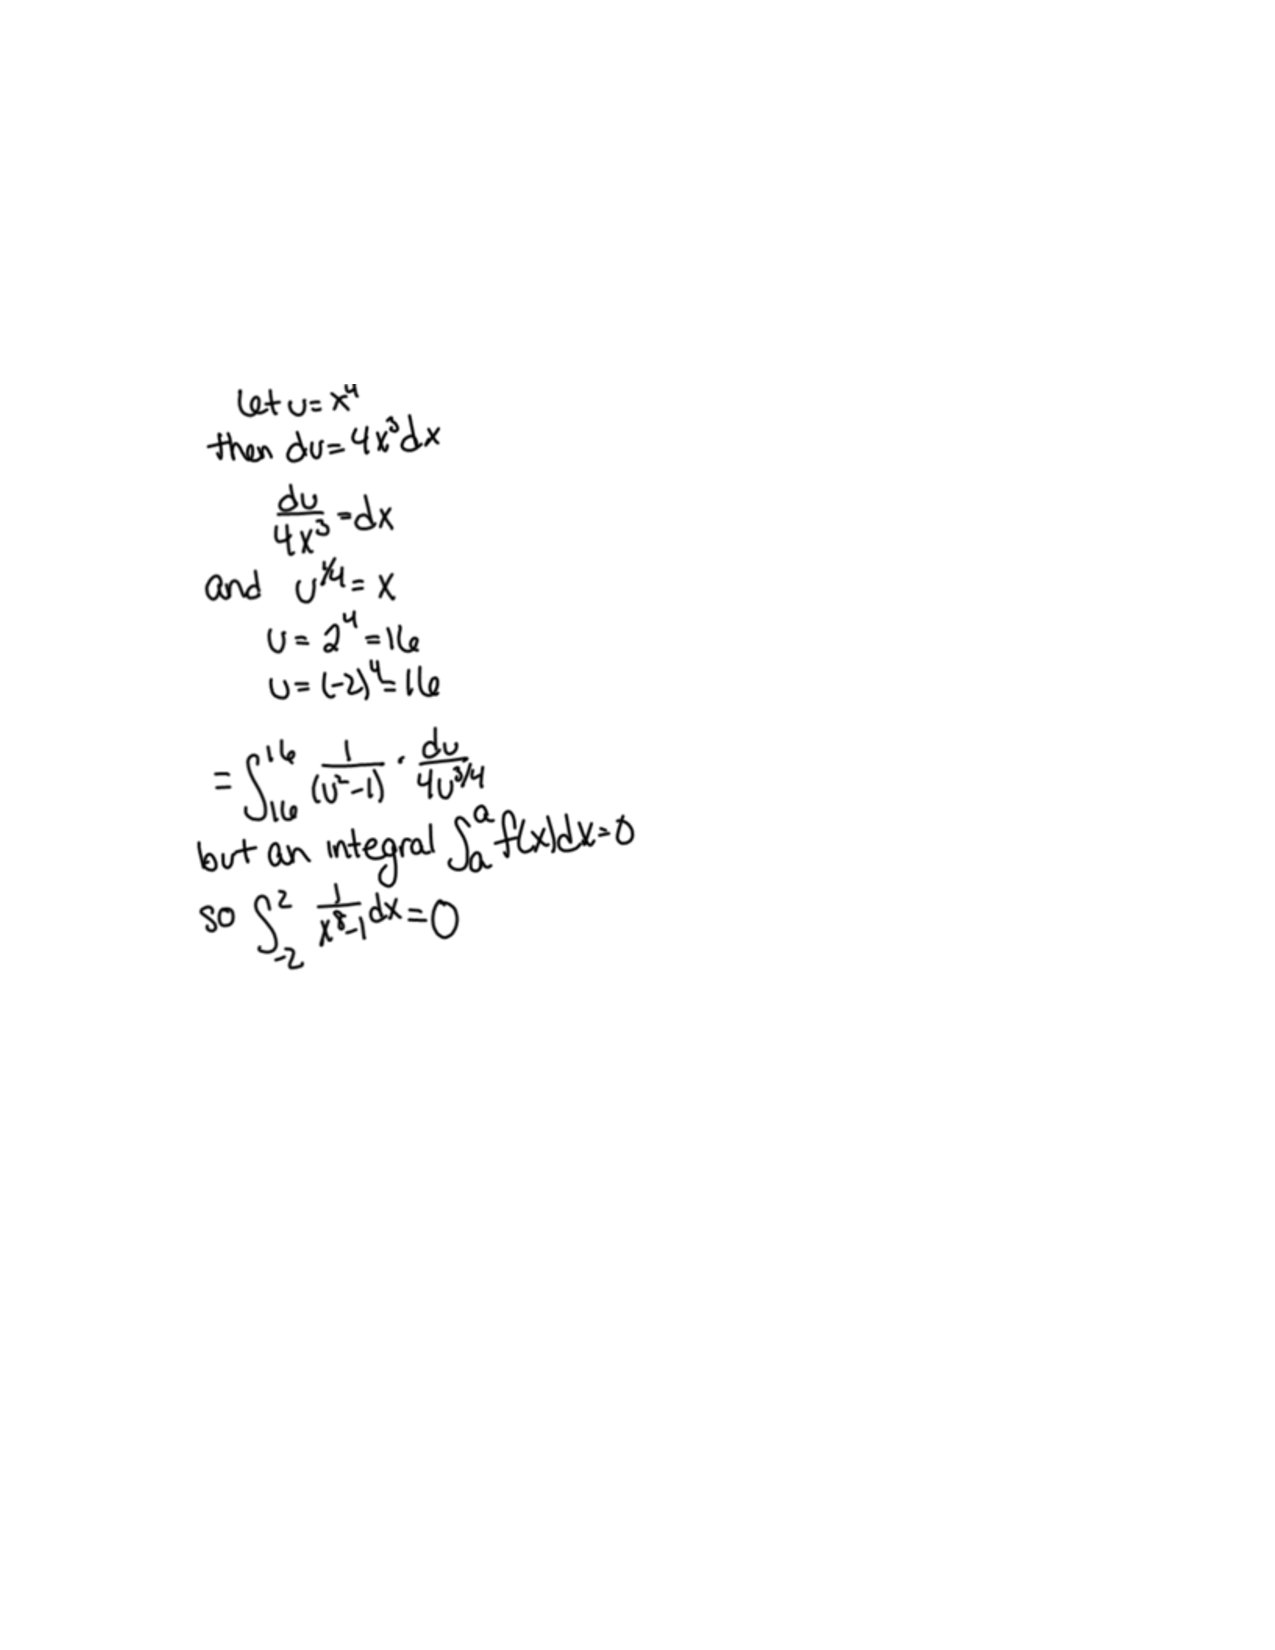
\includegraphics[trim= 170 420 250 180]{Figure1.pdf}
%\end{image}

%add a ``.'' below when used in a specific directory.
\newcommand{\RR}{\mathbb R}
\renewcommand{\d}{\,d}
\newcommand{\dd}[2][]{\frac{d #1}{d #2}}
\renewcommand{\l}{\ell}
\newcommand{\ddx}{\frac{d}{dx}}
\newcommand{\dfn}{\textbf}
\newcommand{\eval}[1]{\bigg[ #1 \bigg]}

\usepackage{multicol}

\renewenvironment{freeResponse}{
\ifhandout\setbox0\vbox\bgroup\else
\begin{trivlist}\item[\hskip \labelsep\bfseries Solution:\hspace{2ex}]
\fi}
{\ifhandout\egroup\else
\end{trivlist}
\fi} %% we can turn off input when making a master document

\title{Recitation \#9: Integration by parts and Trig Integrals}  

\begin{document}
\begin{abstract}		\end{abstract}
\maketitle



\begin{comment}
\section{Warm up:}

	\begin{freeResponse}
	
	\end{freeResponse}
	
\begin{instructorNotes}

\end{instructorNotes}
\end{comment}







\section{Group work:}



%problem 1
\begin{problem}
Evaluate the following integrals
	\begin{enumerate}
	
	\item  $\int_1^3 x^2 5^x \d x$
	\begin{freeResponse}
	We proceed via integration by parts.  Let 
		{\color{red}
		\[
		u = x^2, \qquad \d v = 5^x \d x
		\]
		}
	so that
		{\color{red}
		\[
		\d u = 2x \d x, \qquad v = \frac{5^x}{\ln 5} .
		\]
		}
	Recall the formula for integration by parts is
		\[
		\int_a^b u \d v = \eval{uv}_a^b - \int_a^b v \d u.
		\]
	So we substitute
		\begin{align*}
		\int_1^3 x^2 5^x \d x &= \eval{\frac{x^2 5^x}{\ln(5)}}_1^3 - \int_1^3 2x \frac{5^x}{\ln(5)} \d x  \\
		&= \frac{1}{\ln(5)} \left( 9 \cdot 5^3 - 5 \right) - \frac{2}{\ln(5)} \int_1^3 x 5^x \d x.
		\end{align*}
	For the remaining integral we again use integration by parts:
		{\color{red}
		\[
		u = x, \qquad \d v = 5^x  
		\]
		\[
		\d u = \d x, \qquad v = \frac{5^x}{\ln(5)}.
		\]
		}
	Thus,
		\begin{align*}
		&\frac{1}{\ln(5)} \left( 9 \cdot 5^3 - 5 \right) - \frac{2}{\ln(5)} \int_1^3 x 5^x \d x \\
		&= \frac{5}{\ln(5)} (225 - 1) - \frac{2}{\ln(5)} \left( \eval{\frac{x5^x}{\ln(5)}}_1^3 - \int_1^3 \frac{5^x}{\ln(5)} \d x \right)  \\
		&= \frac{1120}{\ln(5)} - \frac{2}{\ln^2(5)} \left( (3 \cdot 5^3 - 5) - \eval{\frac{5^x}{\ln(5)}}_1^3 \right)  \\
		&= \frac{1}{\ln(5)} \left( 1120 - \frac{740}{\ln(5)} + \frac{248}{\ln^2(5)} \right).
		\end{align*}
	\end{freeResponse}
	
	
	
	\item  $\int \sin(3x) e^{7x} \d x$
	\begin{freeResponse}
	We begin by letting $I = \int \sin(3x) e^{7x} \d x$.  
	We then use integration by parts with
		{\color{red}
		\[
		u = e^{7x} \qquad \d v = \sin(3x) \d x
		\]
		\[
		\d u = 7e^{7x} \d x \qquad v = -\frac{1}{3} \cos(3x).
		\]
		}
	Then
		\begin{align*}
		\int \sin(3x) e^{7x} \d x = I
		&= -\frac{1}{3} e^{7x} \cos(3x) - \int -\frac{1}{3} (7e^{7x}) \cos(3x) \d x  \\
		I &= -\frac{1}{3} e^{7x} \cos(3x) + \frac{7}{3} \int e^{7x} \cos(3x) \d x.
		\end{align*}
	We then apply integration by parts again, this time with
		{\color{red}
		\[
		u = e^{7x} 		\qquad	\d v = \cos(3x) \d x
		\]
		\[
		\d u = 7e^{7x} \d x 	\qquad	v = \frac{1}{3} \sin(3x).
		\]
		}
	This gives us
		\begin{align*}
		I &= -\frac{1}{3} e^{7x} \cos(3x) + \frac{7}{3} \left[ \frac{1}{3} e^{7x} \sin(3x) - \int \frac{1}{3} (7e^{7x}) \sin(3x) \d x \right]  \\
		I &= -\frac{1}{3} e^{7x} \cos(3x) + \frac{7}{9} e^{7x} \sin(3x) - \frac{49}{9} \int e^{7x} \sin(3x) \d x  \\
		I &= -\frac{1}{3} e^{7x} \cos(3x) + \frac{7}{9} e^{7x} \sin(3x) - \frac{49}{9} I  \\
		\frac{58}{9} I &= -\frac{1}{3} e^{7x} \cos(3x) + \frac{7}{9} e^{7x} \sin(3x)  \\
		I &= \frac{9}{58} \left( -\frac{1}{3} e^{7x} \cos(3x) + \frac{7}{9} e^{7x} \sin(3x) \right) + C.
		\end{align*}
	\end{freeResponse}
	
	
	
	\item  $\int x^{\frac{5}{3}} (\ln x)^2 \d x$
	\begin{freeResponse}
	We begin with the substitution
		{\color{red}
		\[
		w = \ln x 	\qquad	\Longrightarrow	\qquad	\d w = \frac{1}{x} \d x, \quad  x = e^w.
		\]}
	Then
		\begin{align*}
		\int x^{\frac{5}{3}} (\ln x)^2 \d x 
		&= \int x^{\frac{8}{3}} (\ln x)^2 \cdot \frac{1}{x} \d x  \\
		&= \int (e^w)^{\frac{8}{3}} w^2 \d w  \\
		&= \int w^2 e^{\frac{8}{3} w} \d w.
		\end{align*}
	We now use integration by parts, with
		{\color{red}
		\[
		u = w^2	\qquad	\d v = e^{\frac{8}{3} w} \d w
		\]
		\[
		\d u = 2w \d w	\qquad	v = \frac{3}{8} e^{\frac{8}{3} w}.
		\]}
	This gives us
		\begin{align*}
		\int x^{\frac{5}{3}} (\ln x)^2 \d x
		&= \frac{3}{8} w^2 e^{\frac{8}{3} w} - \int \frac{3}{8} (2w) e^{\frac{8}{3} w} \d w  \\
		&= \frac{3}{8} w^2 e^{\frac{8}{3} w} - \frac{3}{4} \int w e^{\frac{8}{3} w} \d w.
		\end{align*}
	We apply integration by parts one last time with
	{\color{red}
		\[
		u = w		\qquad	\d v = e^{\frac{8}{3} w} \d w
		\]
		\[
		\d u = \d w	\qquad	v = \frac{3}{8} e^{\frac{8}{3} w}
		\]}
	which yields
		\begin{align*}
		\int x^{\frac{5}{3}} (\ln x)^2 \d x
		&= \frac{3}{8}w^2 e^{\frac{8}{3} w} - \frac{3}{4} \left( \frac{3}{8} w e^{\frac{8}{3} w} - \frac{3}{8} \int e^{\frac{8}{3} w} \d w \right) \\
		&= \frac{3}{8} w^2 e^{\frac{8}{3} w} - \frac{9}{32} w e^{\frac{8}{3} w} + \frac{27}{256} e^{\frac{8}{3} w} + C  \\
		&= \frac{3}{8} e^{\frac{8}{3} \ln x} \left( (\ln x)^2 - \frac{3}{4} \ln x + \frac{9}{32} \right) + C  \\
		&= \frac{3}{8} x^{\frac{8}{3}} \left( (\ln x)^2 - \frac{3}{4} \ln x + \frac{9}{32} \right) + C.
		\end{align*}
	\end{freeResponse}
	
	\end{enumerate}
	
\end{problem}

\begin{instructorNotes}
All three parts involve standard strategies learned in the online lessons.  
For each, split the problems between the groups.  
Then discuss each problem as a class, getting input from the group(s) that worked on that problem.
\end{instructorNotes}







%problem 2
\begin{problem}
Evaluate the following integrals
	\begin{enumerate}
	
	\item  $\int x^5 \cos \left( x^3 \right) \d x$
	\begin{freeResponse}
	We begin with the substitution
		{\color{red}
		\[
		w = x^3 	\qquad	\Longrightarrow	\qquad	\d w = 3x^2 \d x, 	\quad	\frac{1}{3} \d w = x^2 \d x.
		\]
		}
	Then,
		\begin{align*}
		\int x^5 \cos \left( x^3 \right) \d x 
		&= \int x^3 \cos \left( x^3 \right) \cdot x^2 \d x  \\
		&= \int w \cos(w) \cdot \frac{1}{3} \d w  \\
		&= \frac{1}{3} \int w \cos(w) \d w.
		\end{align*}
	We then use integration by parts, with
		{\color{red}
		\[
		u = w 		\qquad	\d v = \cos(w) \d w
		\]
		\[
		\d u = \d w 	\qquad	v = \sin(w)
		\]
		}
	which yields
		\begin{align*}
		\int x^5 \cos \left( x^3 \right) \d x 
		&= \frac{1}{3} \left( w \sin(w) - \int \sin(w) \d w \right)  \\
		&= \frac{1}{3} \left( w \sin(w) + \cos(w) \right) + C  \\
		&= \frac{1}{3} \left( x^3 \sin \left( x^3 \right) + \cos \left( x^3 \right) \right) + C.  
		\end{align*}
	\end{freeResponse}
	
	
	
	\item  $\int \cos \left( \sqrt{x} \right) \d x$
	\begin{freeResponse}
	We begin with the subsitution
		{\color{red}
		\[
		w = \sqrt{x} 	\qquad	\Longrightarrow	\qquad	\d w = \frac{1}{2\sqrt{w}} \d w, \quad	2 \d w = \frac{1}{\sqrt{x}} \d w.
		\]
		}
	Then
		\begin{align*}
		\int \cos \left( \sqrt{x} \right) \d x 
		&= \int \cos \left( \sqrt{x} \right) \cdot \frac{\sqrt{x}}{\sqrt{x}} \d x  \\
		&= 2 \int w \cos(w) \d w  \\
		&= 2 (w \sin(w) + \cos(w)) + C 	\qquad	{\color{red}\text{From part (a)}}  \\
		&=2 \left( \sqrt{x} \sin \left( \sqrt{x} \right) + \cos \left( \sqrt{x} \right) \right) + C.
		\end{align*}
	\end{freeResponse}
	
	
	
	\item  $\int x \cos x \sin x \d x$
	\begin{freeResponse}
	First, recall that
		{\color{red}
		\[
		\sin(2x) = 2 \sin x \cos x 	\qquad	\Longrightarrow	\qquad	\sin x \cos x = \frac{1}{2} \sin(2x).
		\]
		}
	So we can rewrite the given integral as
		\[
		\int x \cos x \sin x \d x = \frac{1}{2} \int x \sin(2x) \d x.
		\]
	Now we use integration by parts with
		{\color{red}
		\[
		u = x 		\qquad	\d v = \sin(2x) \d x
		\]
		\[
		\d u = \d x 	\qquad	v = - \frac{1}{2} \cos(2x).
		\]
		}
	This gives us that
		\begin{align*}
		\frac{1}{2} \int x \sin(2x) \d x
		&= \frac{1}{2} \left( - \frac{1}{2} x \cos(2x) - \int -\frac{1}{2} \cos(2x) \d x \right)  \\
		&= \frac{1}{4} \left( -x \cos(2x) + \frac{1}{2} \sin(2x) \right) + C.
		\end{align*}
	\end{freeResponse}
	
	\end{enumerate}
	
\end{problem}

\begin{instructorNotes}
For this problem, you might just lead a whole class discussion - hopefully soliciting ideas from the students (on their own or with hints).  
You might want to note that some of the problems may be approached in different ways.  
For example, one could begin part (a) with either the substitution $u=x^3$ or by parts with $u=x^3, \d v = x^2 \cos(x^3)$.
\end{instructorNotes}







%problem 3
\begin{problem}
Evaluate the following integrals
	\begin{enumerate}
	
	\item  $\int \tan^{23} x \sec^6 x \d x$
	\begin{freeResponse}
		\begin{align*}
		\int \tan^{23} x \sec^6 x \d x 
		&= \int \tan^{23} x \sec^4 x \sec^2 x \d x  \\
		&= \int \tan^{23} x \left( 1 + \tan^2 x \right)^2 \sec^2 x \d x .
		\end{align*}
	We now substitute
		{\color{red}
		\[
		u = \tan x 	\qquad	\Longrightarrow		\qquad	\d u = \sec^2 x \d x.
		\]
		}
	Then
		\begin{align*}
		\int \tan^{23} x \left( 1 + \tan^2 x \right)^2 \sec^2 x \d x
		&= \int u^{23} (1+u^2)^2 \d u  \\
		&= \int u^{23} (1 + 2u^2 + u^4) \d u  \\
		&= \int \left( u^{23} + 2u^{25} + u^{27} \right) \d u  \\
		&= \frac{1}{24} u^{24} + \frac{1}{13} u^{26} + \frac{1}{28} u^{28} + C  \\
		&= \frac{1}{24} \tan^{24} x + \frac{1}{13} \tan^{26} x + \frac{1}{28} \tan^{28} x + C.
		\end{align*}
	\end{freeResponse}
	
	
	
	\item  $\int \tan^2 x \sec x \d x$ \qquad {\color{red} Hint:  $\int \sec x \d x = \ln | \sec x \tan x| + C$}
	\begin{freeResponse}
		\begin{align}
		\int \tan^2 x \sec x \d x
		&= \int \left( \sec^2 x - 1 \right) \sec x \d x  \nonumber	\\
		&= \int \sec^3 x \d x - \int \sec x \d x  		\nonumber	\\
		&= \int \sec^3 x \d x - \ln | \sec x \tan x| 	\qquad	{\color{red}\text{from the hint}}	\label{equation 1}
		\end{align}
	Now, in an attempt to evaluate $\int \sec^3 x \d x$, we use integration by parts with
		{\color{red}
		\[
		u = \sec x 				\qquad	\d v = \sec^2 x \d x
		\]
		\[
		\d u = \sec x \tan x \d x	\qquad	v = \tan x.
		\]
		}
	So
		\begin{equation}\label{equation 2}
		\int \sec^3 x \d x = \sec x \tan x - \int \tan^2 x \sec x \d x.
		\end{equation}
	Combining equations \eqref{equation 1} and \eqref{equation 2} yields
		\begin{align*}
		\int \tan^2 x \sec x \d x &= \int \sec^3 x \d x - \ln | \sec x \tan x|   \\
		\int \tan^2 x \sec x \d x &= \sec x \tan x - \int \tan^2 x \sec x \d x - \ln | \sec x \tan x |  \\
		2 \int \tan^2 x \sec x \d x &= \sec x \tan x - \ln | \sec x \tan x | + C  \\
		\int \tan^2 x \sec x \d x &= \frac{1}{2} \left( \sec x \tan x - \ln | \sec x \tan x | \right) + C.
		\end{align*}
	\end{freeResponse}
	
	
	
	\item  $\int \tan^2 x \sin x \d x$
	\begin{freeResponse}
		\begin{align*}
		\int \tan^2 x \sin x \d x
		&= \int \frac{\sin^2 x}{\cos^2 x} \sin x \d x  \\
		&= \int \frac{1-\cos^2 x}{\cos^2 x} \sin x \d x.
		\end{align*}
	Now we substitute
		{\color{red}
		\[
		u = \cos x 		\qquad	\Longrightarrow		\qquad	\d u = - \sin x \d x, \quad - \d u = \sin x \d x.
		\]
		}
	This gives us that
		\begin{align*}
		\int \tan^2 x \sin x \d x
		&= \int \frac{1-u^2}{u^2} (-1) \d u  \\
		&= \int \frac{u^2 - 1}{u^2} \d u  \\
		&= \int \left( 1 - u^{-2} \right) \d u  \\
		&= u + \frac{1}{u} + C  \\
		&= \cos x + \sec x + C.
		\end{align*}
	\end{freeResponse}
	
	\end{enumerate}
	
\end{problem}

\begin{instructorNotes}
All three parts involve standard strategies learned in the online lessons.  
For each, split the problems between the groups.  
Then discuss each problem as a class, getting input from the group(s) that worked on that problem.
\end{instructorNotes}







%problem 4
\begin{problem}
Evaluate
	\[
	\int_{- \pi}^0 \sqrt{1 - \cos^2 x} \d x.
	\]
	\begin{freeResponse}
		\begin{align*}
		\int_{- \pi}^0 \sqrt{1 - \cos^2 x} \d x
		&= \int_{- \pi}^0 \sqrt{\sin^2 x} \d x  \\
		&= \int_{- \pi}^0 | \sin x | \d x.
		\end{align*}
	Now, when $-\pi \leq x \leq 0$, $\sin x \leq 0$.  
	Thus, on this region, $|\sin x | = - \sin x$.
	So we continue
		\begin{align*}
		\int_{- \pi}^0 \sqrt{1 - \cos^2 x} \d x
		&= \int_{- \pi}^0 - \sin x \d x  \\
		&= \eval{\cos x}_{-\pi}^0  \\
		&= \cos(0) - \cos(-\pi) = 1 - (-1) = 2.
		\end{align*}
	\end{freeResponse}
		
\end{problem}

\begin{instructorNotes}
You may want to do this problem as a whole class - perhaps play-acting by claiming that it is equal to $\int_{-\pi}^0 \sin x \d x$ rather than $\int_{-\pi}^0 \left| \sin x \right|  \d x$
\end{instructorNotes}

















	
	
	
	
	
	
	
	
	

	










								
				
				
	














\end{document} 


















